\documentclass[11pt,a4paper]{article}

\usepackage[T1]{fontenc}
\usepackage[utf8]{inputenc}
\usepackage{lmodern}
\usepackage{microtype}
\usepackage[margin=2.4cm]{geometry}
\usepackage{amsmath,amssymb}
\usepackage{graphicx}
\usepackage{booktabs}
\usepackage{tabularx}
\usepackage{array}
\usepackage{xcolor}
\usepackage{caption}
\usepackage{subcaption}
\usepackage{enumitem}
\usepackage{tikz}
\usetikzlibrary{arrows.meta,positioning,fit,backgrounds,calc}
\usepackage[hidelinks]{hyperref}

\graphicspath{{figures/}}
\setlist{itemsep=2pt,topsep=4pt}
\captionsetup{font=small,labelfont=bf}
\newcommand{\code}[1]{\texttt{#1}}
\newcommand{\best}[1]{\textbf{#1}}

\title{Probabilistic Day-Ahead Electricity Price Forecasting\\for the Swedish Bidding Zones SE1--SE4\\[4pt]
\large Process, decisions and results: milestones M0--M5 and M8}
\author{Pipeline \code{pricefc} \quad\textperiodcentered\quad
\href{https://github.com/saldestechnology/ml-electro-mlops}{saldestechnology/ml-electro-mlops}}
\date{5 October 2026}

\begin{document}
\maketitle

\begin{abstract}
\noindent
We built a fully versioned pipeline that forecasts hourly day-ahead electricity prices for the four
Swedish bidding zones, issued at 09:00 Europe/Stockholm on day $D$ for every hour of $D{+}1$, as
seven quantiles. All data, datasets, models and evaluations are tracked in MLflow with lineage back
to immutable raw snapshots and the git commit. Every input carries an explicit availability rule
and every dataset build passes an automated leakage audit. Over a one-year out-of-sample backtest
(3 Oct 2025 -- 2 Oct 2026, true-lead weather forecasts), a tuned and recalibrated LightGBM quantile
model beats the strongest classical baseline (MSTL+ETS) in every zone by 0.78--1.43~EUR/MWh mean
pinball loss (13--23\%), with block-bootstrap confidence intervals that exclude zero. The
pretrained foundation model TimesFM~3.0 with weather and calendar covariates is better still
(a further 12--20\% over LightGBM, significant in every zone), but its weights are licensed for
non-commercial use only, so it serves as a benchmark rather than a deployable model. The
deployable TimesFM~2.5 is weaker than LightGBM overall, yet makes complementary errors (it halves
the night-hour error). An ensemble of the two deployable models, with weights per hour of the
delivery day learnt only from past forecasts, improves on LightGBM by a further 5--9\% in every
zone (significant everywhere), closing 28--65\% of the gap to the non-deployable benchmark. It is
the champion candidate.
\end{abstract}

\tableofcontents

%------------------------------------------------------------------------------
\section{Problem and scope}

\paragraph{Forecasting task.}
Nordic day-ahead prices for delivery day $D{+}1$ are set in the SDAC auction at noon CET on day
$D$ and published around 12:45--13:00. A forecast that is useful for bidding must therefore be
issued \emph{before} the auction: our origin is 09:00 Europe/Stockholm on day $D$, and the target
is every hour of local day $D{+}1$ (23, 24 or 25 hours, depending on daylight-saving changes).
Forecasts are probabilistic: quantiles $\tau \in \{0.05, 0.10, 0.25, 0.50, 0.75, 0.90, 0.95\}$.

\paragraph{Zones and resolution.}
Sweden has four bidding zones with separate prices: SE1 (north) to SE4 (south, most coupled to the
continent and the most volatile). On 1 October 2025 the market moved from hourly to 15-minute
market time units; we aggregate to hourly means so the series stays homogeneous, and record the
source resolution per row.

\paragraph{Constraints.}
Work proceeds in milestones (M0 skeleton, M1 ingestion, M2 datasets, M3 backtesting and baselines,
M4 LightGBM, M5 TimesFM, M6 registry and serving, M7 cloud GPU, M8 ensembles). All computation
so far ran on a laptop (Apple M1 Pro, 32~GB). A \$25 RunPod GPU budget is reserved for
foundation-model fine-tuning and may only be spent with the owner's explicit approval; none has
been spent.

%------------------------------------------------------------------------------
\section{Architecture and engineering principles}

\begin{figure}[h]
\centering
\resizebox{\linewidth}{!}{%
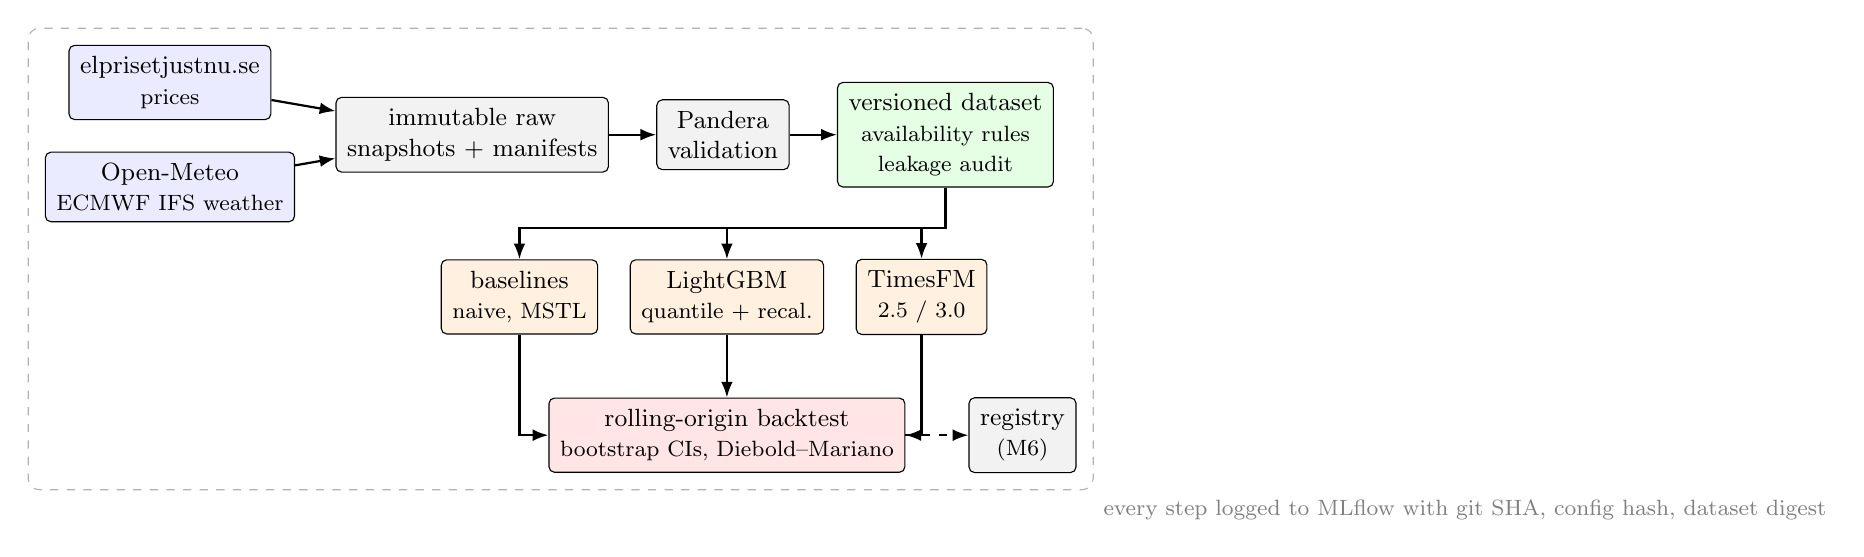
\begin{tikzpicture}[
  box/.style={draw,rounded corners=2pt,fill=#1,minimum height=8mm,align=center,font=\small,inner sep=4pt},
  box/.default=white,
  arr/.style={-{Latex[length=2mm]},thick}]
\node[box=blue!8] (ep) {elprisetjustnu.se\\\footnotesize prices};
\node[box=blue!8,below=4mm of ep] (om) {Open-Meteo\\\footnotesize ECMWF IFS weather};
\node[box=gray!10] (raw) at ($(ep.east)!0.5!(om.east)+(24mm,0)$) {immutable raw\\snapshots + manifests};
\node[box=gray!10,right=6mm of raw] (val) {Pandera\\validation};
\node[box=green!10,right=6mm of val] (ds) {versioned dataset\\\footnotesize availability rules\\\footnotesize leakage audit};
\node[box=orange!12,below=11mm of raw,xshift=6mm] (bl) {baselines\\\footnotesize naive, MSTL};
\node[box=orange!12,right=4mm of bl] (lg) {LightGBM\\\footnotesize quantile + recal.};
\node[box=orange!12,right=4mm of lg] (tf) {TimesFM\\\footnotesize 2.5 / 3.0};
\node[box=red!10,below=8mm of lg] (bt) {rolling-origin backtest\\\footnotesize bootstrap CIs, Diebold--Mariano};
\node[box=gray!10,right=8mm of bt] (reg) {registry\\\footnotesize (M6)};
\draw[arr] (ep) -- (raw); \draw[arr] (om) -- (raw);
\draw[arr] (raw) -- (val); \draw[arr] (val) -- (ds);
\draw[arr] (ds) |- ($(lg.north)+(0,4mm)$) -| (bl.north);
\draw[arr] ($(lg.north)+(0,4mm)$) -- (lg.north);
\draw[arr] ($(lg.north)+(0,4mm)$) -| (tf.north);
\draw[arr] (bl.south) |- (bt.west); \draw[arr] (lg) -- (bt); \draw[arr] (tf.south) |- (bt.east);
\draw[arr,dashed] (bt) -- (reg);
\begin{scope}[on background layer]
\node[draw=gray!60,dashed,rounded corners,fit=(ep)(om)(raw)(val)(ds)(bl)(lg)(tf)(bt)(reg),inner sep=6pt,
  label={[font=\footnotesize,gray]south east:every step logged to MLflow with git SHA, config hash, dataset digest}] {};
\end{scope}
\end{tikzpicture}}
\caption{Pipeline overview. Solid arrows exist today; the registry is milestone M6.}
\label{fig:pipeline}
\end{figure}

\begin{itemize}
\item \textbf{Reproducibility.} Python 3.12 managed by \code{uv} with a committed lockfile; YAML
configs validated by strict pydantic models and hashed; MLflow (SQLite backend) with required
tags on every run: zone, resolution, weather source, dataset version, git SHA and dirty flag,
model family, compute environment, config hash and pipeline stage.
\item \textbf{Immutability.} Raw pulls are written read-only, one directory per source,
dataset, key and pull time, with a manifest (request, row
counts, hashes, validation result, git SHA). Snapshots are never overwritten; invalid ones are kept
and marked, so the record of what an API returned is preserved.
\item \textbf{Quality gates.} GitHub Actions runs \code{ruff}, \code{mypy --strict} and
\code{pytest} (124 offline tests, including Hypothesis property tests) on every push; live API
tests are opt-in.
\item \textbf{Scale.} 34 commits, about 5{,}400 lines of library code and 2{,}000 lines of tests.
\end{itemize}

%------------------------------------------------------------------------------
\section{Data (M1)}

\subsection{Prices}
The specification named ENTSO-E as the source of record. Its API token requires a manual
application, and the owner decided not to apply. We therefore made the price source pluggable
(\code{PriceSource}) and adopted \textbf{elprisetjustnu.se}, which publishes one JSON file per
zone and local day from 1 November 2021, in EUR/kWh without VAT.

Practical issues found and handled:
\begin{itemize}
\item The default Python user agent receives HTTP 403; the client sends its own.
\item \code{time\_end} is computed in wall-clock time, so the last slot before the autumn DST
change claims 75 minutes. Resolution is derived from the spacing of \code{time\_start} instead,
and anomalies are recorded in the manifest.
\item Snapshots are per zone and month; ingest resumes by skipping complete, valid months.
\end{itemize}

\paragraph{Verification against independent sources.}
Before trusting the series we compared it with Nord Pool (40 zone-days, 3{,}840 quarter-hours:
identical to the cent) and with Energy-Charts (12 stress days $\times$ 4 zones including DST days
in both resolution eras, the market-time-unit switch and the 2022 crisis peak: 47 of 48 zone-days
identical). Energy-Charts' licence permits private use only, so it was used for this check and
never as a data source.

The one mismatch exposed a \textbf{source defect}: on five days (SE3 2021-11-04; SE2 2022-09-04,
09-10, 09-15, 10-20) the source dropped one hour and shifted every later hour one slot earlier,
with errors up to 139~EUR/MWh. Validation caught all five (23 rows on a 24-hour day). These values
are wrong rather than incomplete, so they are \emph{never repaired}: a \code{known\_bad\_days}
list drops them at ingest while still recording how many rows the source returned, so a later
correction would be visible.

\begin{figure}[h]
\centering
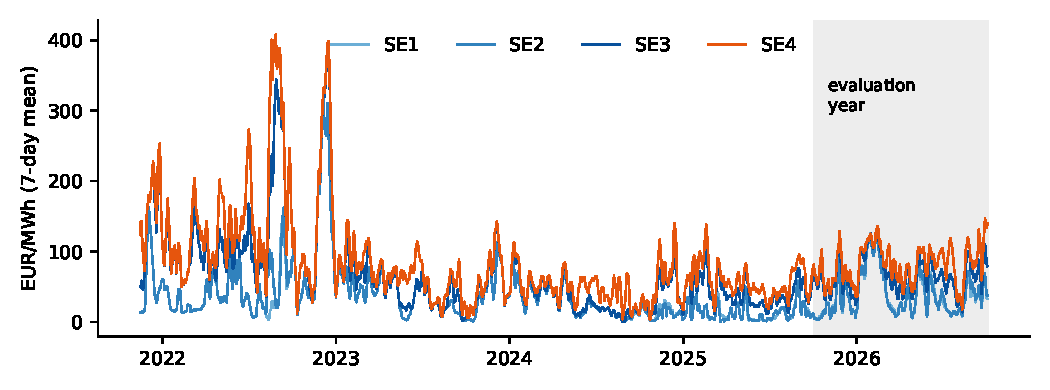
\includegraphics[width=\linewidth]{prices}
\caption{Daily mean day-ahead price (7-day rolling mean), all zones. The 2022 energy crisis
dominates the early history; the shaded year is the out-of-sample evaluation window.}
\label{fig:prices}
\end{figure}

\subsection{Weather}
Weather comes from Open-Meteo, pinned to the \textbf{ECMWF IFS} model. The default
\code{best\_match} silently switches between underlying models and lacks 100\,m wind in the
archive, which would break reproducibility. Two endpoints are used:
\begin{itemize}
\item \emph{Historical Forecast} (2021 onwards): a ``stitched'' series of short-range forecasts,
used for training. Its exact issue time is unknown.
\item \emph{Previous Runs} (from 1--2 October 2025): forecasts as they were issued $N$ days ahead.
This is what a live system would have had, so it is used for evaluation.
\end{itemize}
Each zone uses 3--5 locations (SE4 includes Danish and German points), eight variables, plus
zone-level aggregates. The Previous Runs archive has gaps between late March and early May 2026,
which validation tolerates per endpoint (\code{max\_null\_frac}) and records per column; nothing is
imputed silently.

%------------------------------------------------------------------------------
\section{Datasets and leakage control (M2)}

\subsection{Availability rules}
Every input source declares when each value becomes known, and feature builders only see an
\emph{as-of} view of the data at the origin:
\begin{itemize}
\item \textbf{Prices} for delivery day $X$ are known from $X{-}1$ 13:00 local time (conservative
relative to the 12:45 publication). At the origin, prices up to the end of day $D$ are therefore
known; those of $D{+}1$ are the target.
\item \textbf{Weather} valid at time $T$ is known from $T - 48\,\mathrm{h} + 8\,\mathrm{h}$
(day-2 lead plus publication delay). Open-Meteo defines the day-1 lead as issued $24$\,h before
the valid time; with the delay it would arrive \emph{after} the origin for most hours of $D{+}1$,
so the stricter day-2 lead is used.
\end{itemize}

\subsection{Leakage audit}
Every dataset build runs an audit: for seeded random origins, both ends of the range and every
origin whose target day has 23 or 25 hours, all data that is unavailable at the origin is
perturbed and every feature must stay bit-identical. The perturbation must also change the target,
so the test cannot pass vacuously. A build that fails the audit is rejected. A Hypothesis property
test and deliberately injected leaks (which the audit must catch) guard the audit itself. Later we
added a second guard: the backtest harness strips the target and its metadata before calling a
model's \code{predict}, enforced by a test.

\subsection{Features and versioning}
Rows are (origin day, target hour). Features: calendar (hour, weekday, Swedish public, de facto
and half holidays, bridge days, DST), own-price lags and rolling statistics up to the end of day
$D$, neighbouring-zone prices, and weather at each location plus zone aggregates (108 features for
SE3). Datasets are stored as
\code{data/datasets/\{zone\}/hourly/\{date\}-\{digest\}/} with a lineage manifest listing every
contributing raw snapshot, and logged to MLflow as dataset inputs.

\paragraph{A locale bug caught by CI.}
The \code{holidays} package localises holiday names from the system locale, and the calendar code
matched on English names. Under a C or Swedish locale every Sunday became a public holiday. The
language is now pinned and a test builds the calendar under three locales.

\subsection{The train/evaluation weather gap}
Training uses the stitched weather series, evaluation the true day-2 forecasts. On the overlapping
SE3 year they agree closely for temperature ($r=0.996$) and radiation ($r=0.991$) but less for
100\,m wind ($r=0.939$, MAE 0.6\,m/s), the most price-relevant variable
(Figure~\ref{fig:weather}). Models trained on the stitched series should therefore be expected to
be over-confident in evaluation, which is exactly what we later observed (Section~\ref{sec:calib}).

\begin{figure}[h]
\centering
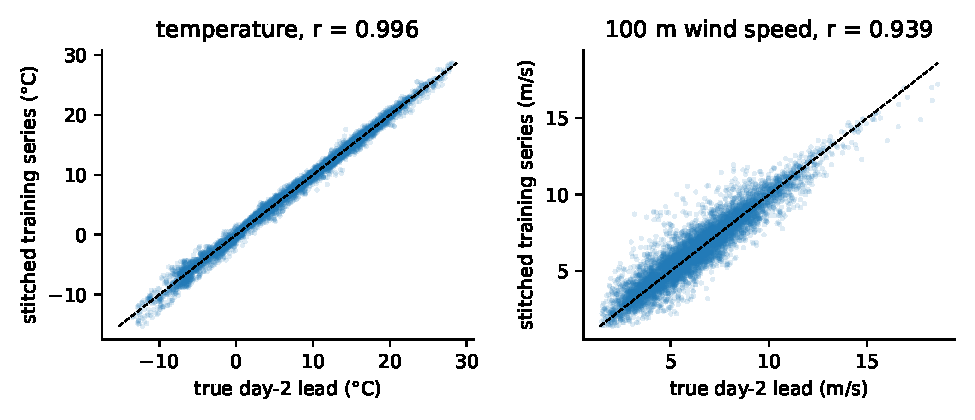
\includegraphics[width=0.85\linewidth]{weather_gap}
\caption{Stitched training weather versus the true day-2 forecast (SE3 zone means, one year).}
\label{fig:weather}
\end{figure}

%------------------------------------------------------------------------------
\section{Evaluation methodology (M3)}

\paragraph{Rolling-origin backtest.}
For each of the 365 origins from 3 October 2025 to 2 October 2026, models are trained on stitched
rows whose target day is at most $D$ (i.e.\ published before the origin) and predict the true-lead
rows of $D{+}1$. Models refit monthly by default; models that need the most recent history refit
at every origin. Quantile crossings are repaired by sorting.

\paragraph{Metrics.}
The primary metric is the pinball loss averaged over the seven quantiles,
\begin{equation}
L_\tau(y, q) = \max\bigl(\tau (y-q),\; (\tau-1)(y-q)\bigr), \qquad
\bar L = \frac{1}{|\mathcal T|}\sum_{\tau\in\mathcal T} \operatorname{mean}_t L_\tau(y_t, q_{\tau,t}),
\end{equation}
complemented by MAE of the median, bias, sMAPE (denominator floored at 1~EUR/MWh because of
negative prices), empirical coverage of the 80\% and 90\% intervals, and slices by hour, weekday,
season, spike days and negative-price hours.

\paragraph{Statistical comparison.}
Losses are aggregated per day. Confidence intervals come from a circular block bootstrap
(7-day blocks, 2{,}000 resamples) of the daily mean loss and of paired daily differences between
two models. The Diebold--Mariano test with the Harvey--Leybourne--Newbold small-sample correction
is applied to the daily loss differential $d_t$:
\begin{equation}
\mathrm{DM} = \frac{\bar d}{\sqrt{\hat\gamma_0 / n}}, \qquad
\mathrm{DM}_{\mathrm{HLN}} = \mathrm{DM}\,\sqrt{\frac{n+1-2h+h(h-1)/n}{n}}, \quad h=1,
\end{equation}
compared with a $t_{n-1}$ distribution.

\paragraph{Lesson: biased development samples.}
A quick development mode evaluates every $k$-th origin. With $k=7$ every target was a Saturday,
which reversed the ranking of the 1-day and 7-day naive models. The default is now $k=5$, and
multiples of 7 are rejected by config validation. A second lesson came later (M5): a 73-origin
development sample ranked TimesFM~2.5 level with LightGBM, whereas the full year showed it clearly
worse in three zones. Decisions are only taken on full-year runs.

\paragraph{Baselines.}
Seasonal naive (same hour 7 days and 1 day earlier), the EPF ``weekday'' naive, and
StatsForecast MSTL with daily and weekly seasonality and an AutoETS trend (56-day context).
Naive quantiles are empirical per-hour quantiles of each method's own recent errors.
Table~\ref{tab:baselines} shows that MSTL is much stronger than the naive methods; it became the
bar for M4.

\begin{table}[h]
\centering\small
\caption{Baselines, 365 origins: mean pinball loss (EUR/MWh) with 95\% block-bootstrap CI for
MSTL, and MSTL skill relative to the 7-day naive reference.}
\label{tab:baselines}
\begin{tabular}{lccccc}
\toprule
Zone & MSTL+ETS & Naive 1d & Weekday naive & Naive 7d & MSTL skill\\
\midrule
SE1 & 5.95 (5.31--6.65) & 7.70 & 8.41 & 11.12 & 0.47\\
SE2 & 6.22 (5.53--6.97) & 8.02 & 8.80 & 11.48 & 0.46\\
SE3 & 6.53 (6.09--6.98) & 9.15 & 9.16 & 11.61 & 0.44\\
SE4 & 8.35 (7.63--9.14) & 11.41 & 11.52 & 13.69 & 0.39\\
\bottomrule
\end{tabular}
\end{table}

%------------------------------------------------------------------------------
\section{LightGBM quantile model (M4)}

\subsection{Model and tuning}
One LightGBM regressor per quantile with the quantile objective, on all dataset features. Hyper-
parameters were tuned per zone with Optuna (seeded TPE sampler, median pruner, 40 trials) on four
expanding-window folds of 91 days that all end \emph{before} the evaluation year; the code asserts
that tuning never touches the evaluation window. The objective is mean pinball loss over
$\tau\in\{0.1,0.5,0.9\}$, and the number of trees is the median early-stopping iteration of the best
trial. Interestingly, SE3 prefers large trees (252 leaves), whereas SE1, SE2 and SE4 prefer small,
heavily regularised trees (17--29 leaves). Tuning improved SE3 only modestly over sensible defaults
($-0.09$~EUR/MWh, CI $[-0.19, +0.005]$).

\begin{figure}[h]
\centering
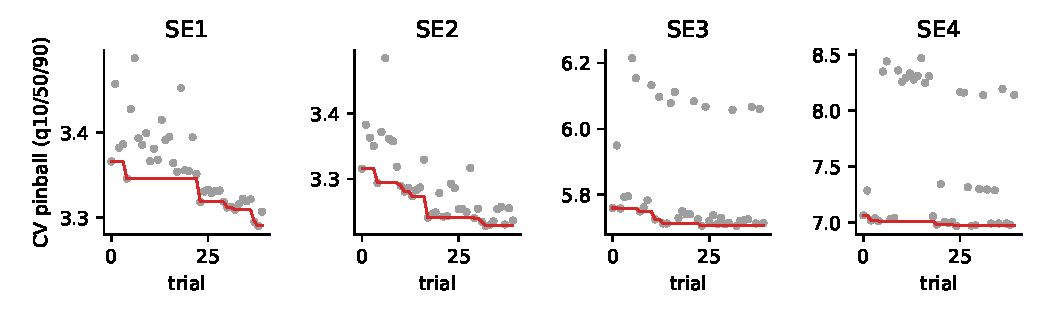
\includegraphics[width=\linewidth]{hpo}
\caption{Optuna studies: cross-validated pinball loss per trial (grey) and best so far (red).}
\label{fig:hpo}
\end{figure}

\subsection{Over-confidence and recalibration}
\label{sec:calib}
On true-lead data the raw model was over-confident: its 80\% and 90\% intervals covered only
72\% and 84\% of SE3 prices, and the median ran 5.7~EUR/MWh low. This matches the weather gap of
Figure~\ref{fig:weather}: the model learned from more accurate weather than it receives live.
We added a model-agnostic wrapper that, at every origin, shifts each quantile by the
$\tau$-quantile of the model's own residuals over the last 28 published days:
\begin{equation}
\hat q^{\,\mathrm{cal}}_{\tau} = \hat q_{\tau} + Q_\tau\bigl(\{ y_s - \hat q_{\tau,s} :
s \text{ in the last 28 published days}\}\bigr).
\end{equation}
Only realised prices that are published before the origin enter the offsets. Coverage moved to
77.6\%/87.9\% and the pinball loss improved slightly (Figure~\ref{fig:reliability}); a 14-day
window was too noisy. The first week of a deployment is uncalibrated (cold start).

\begin{figure}[h]
\centering
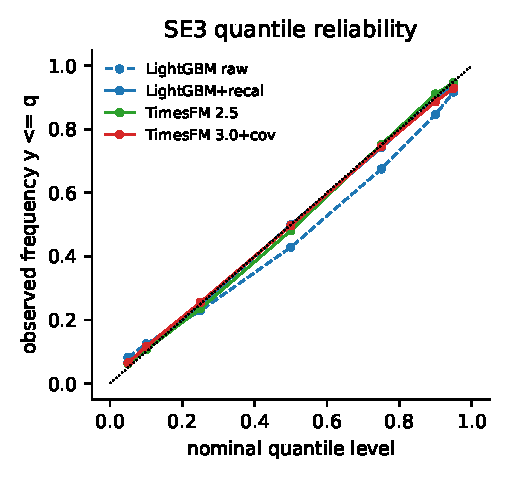
\includegraphics[width=0.48\linewidth]{reliability}
\caption{Reliability of the SE3 quantiles: the fraction of prices below each forecast quantile
versus its nominal level. The dashed line is raw LightGBM.}
\label{fig:reliability}
\end{figure}

\subsection{Results}
Recalibrated LightGBM beats MSTL in every zone (Table~\ref{tab:lgbm}). Further checks on SE3:
\begin{itemize}
\item \textbf{Seed variance}: six seeds give $5.730 \pm 0.009$, about 100 times smaller than the
margin over MSTL.
\item \textbf{Crisis years}: training only from July 2023 is clearly worse (6.09 vs 5.75), so
the 2021--2023 crisis history is kept.
\item \textbf{Importance}: own price history 55\% of gain (the price 24 hours earlier alone 26\%),
weather 27\% with 100\,m wind leading, calendar 12\%, neighbouring zones 6\%
(Figure~\ref{fig:importance}).
\item \textbf{Remaining weakness}: the median still under-forecasts by 2--4~EUR/MWh on average;
the residual-quantile offset does not target mean bias and price spikes pull the mean above the
median.
\end{itemize}

\begin{table}[h]
\centering\small
\caption{LightGBM, 365 origins per zone: mean pinball loss (EUR/MWh), paired difference to MSTL with
95\% block-bootstrap CI, Diebold--Mariano p-value, interval coverage and median bias.}
\label{tab:lgbm}
\footnotesize\setlength{\tabcolsep}{3.5pt}
\begin{tabular}{lcccccccc}
\toprule
Zone & LGBM+recal & LGBM raw & MSTL & Naive 7d & $\Delta$ vs MSTL [95\% CI] & DM $p$ & Cov.\ 80/90 & Bias\\
\midrule
SE1 & \best{5.053} & 5.060 & 5.950 & 11.117 & $-0.90$ [$-1.26$, $-0.54$] & $2\cdot10^{-7}$ & 76.9/88.3 & $-3.4$\\
SE2 & \best{4.788} & 4.790 & 6.216 & 11.479 & $-1.43$ [$-1.75$, $-1.11$] & $7\cdot10^{-15}$ & 78.4/88.8 & $-4.0$\\
SE3 & \best{5.727} & 5.753 & 6.530 & 11.613 & $-0.78$ [$-1.15$, $-0.40$] & $<10^{-3}$ & 77.6/87.9 & $-2.1$\\
SE4 & \best{6.920} & 7.011 & 8.351 & 13.691 & $-1.43$ [$-1.89$, $-1.00$] & $8\cdot10^{-12}$ & 77.7/88.7 & $-1.7$\\
\bottomrule
\end{tabular}
\end{table}

\begin{figure}[h]
\centering
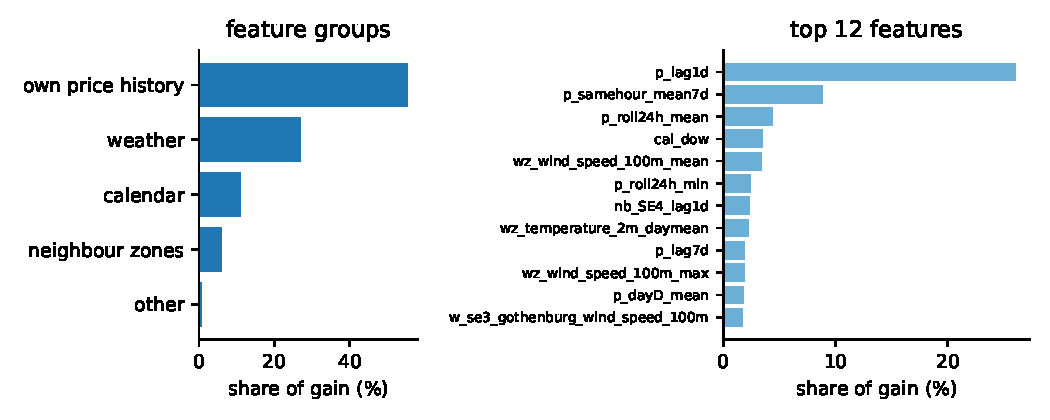
\includegraphics[width=\linewidth]{importance}
\caption{SE3 LightGBM feature importance (gain of the median model, averaged over monthly refits).}
\label{fig:importance}
\end{figure}

By the promotion criteria of the specification (better mean pinball than the incumbent, paired CI
excluding zero or significant DM test, coverage within tolerance, clean leakage audit), the
recalibrated LightGBM is the champion candidate in every zone. Formal registration requires the
model wrapper of M6.

%------------------------------------------------------------------------------
\section{Foundation model TimesFM (M5)}

\subsection{Versions and licensing}
Checking the current release before building (as the specification requires) found two relevant
checkpoints, both pinned by Hugging Face revision hash:
\begin{itemize}
\item \textbf{TimesFM 2.5} (200M parameters, Apache-2.0): context up to 16k points, decile
outputs, covariates through ``XReg'' (an in-context linear regression, with TimesFM forecasting
its residuals).
\item \textbf{TimesFM 3.0} (released August 2026): native past and future covariates and an MLX
backend for Apple silicon. Its weights are licensed for \emph{non-commercial, non-production use
only}, and fine-tuned versions are derivatives under the same terms.
\end{itemize}
The owner decided to evaluate 2.5 as the deployable candidate and 3.0 as a research benchmark.
The adapter refuses to load 3.0 unless \code{accept\_noncommercial\_licence} is set, and its runs
are tagged \code{deployable=false} so they can never be promoted.

\subsection{Adapter}
TimesFM plugs into the same harness as every other model. At each origin the context is the last
2{,}048 published hours (ending at local midnight before $D{+}1$), and the forecast covers exactly
the target hours. Covariates are the zone-mean temperature, 100\,m wind, radiation and cloud cover
plus calendar features; their future values come from the leakage-audited feature rows. TimesFM
emits deciles, which are linearly interpolated to our quantile levels, with the 5\% and 95\% tails
extrapolated from the median using normal-distribution scaling.

Smoke tests on the laptop: 2.5 takes 0.24\,s per forecast on CPU (the Apple GPU was slower);
3.0 on MLX takes 0.05\,s. A full-year backtest takes 1.5--5 minutes per model, so no GPU was
needed. Two problems surfaced: TimesFM~2.5 clamps forecasts at zero whenever the context has no
negative prices unless \code{infer\_is\_positive} is disabled, and torch inference
\emph{deadlocked} after a LightGBM fit in the same process, because the two libraries bundle
separate copies of the OpenMP runtime on macOS. Restricting torch to one thread removed the
deadlock at little cost.

\subsection{Results}

\begin{table}[h]
\centering\small
\caption{TimesFM versus recalibrated LightGBM, 365 origins per zone: mean pinball loss (EUR/MWh)
and paired difference to LightGBM with 95\% block-bootstrap CI.}
\label{tab:timesfm}
\setlength{\tabcolsep}{4pt}
\begin{tabular}{lcccccc}
\toprule
& & \multicolumn{2}{c}{TimesFM 3.0 + covariates} & & \multicolumn{2}{c}{TimesFM 2.5 (deployable)}\\
\cmidrule(lr){3-4}\cmidrule(lr){6-7}
Zone & LGBM+recal & pinball & $\Delta$ [95\% CI] & TimesFM 3.0 & pinball & $\Delta$ [95\% CI]\\
\midrule
SE1 & 5.053 & \best{4.054} & $-1.00$ [$-1.28$, $-0.72$] & 4.792 & 4.927 & $-0.13$ [$-0.42$, $+0.19$]\\
SE2 & 4.788 & \best{3.866} & $-0.92$ [$-1.21$, $-0.66$] & 5.082 & 5.188 & $+0.40$ [$+0.14$, $+0.67$]\\
SE3 & 5.727 & \best{4.989} & $-0.74$ [$-1.01$, $-0.45$] & 5.757 & 6.118 & $+0.39$ [$+0.07$, $+0.71$]\\
SE4 & 6.920 & \best{6.059} & $-0.86$ [$-1.11$, $-0.62$] & 7.110 & 7.505 & $+0.59$ [$+0.24$, $+0.95$]\\
\bottomrule
\end{tabular}
\end{table}

\begin{figure}[h]
\centering
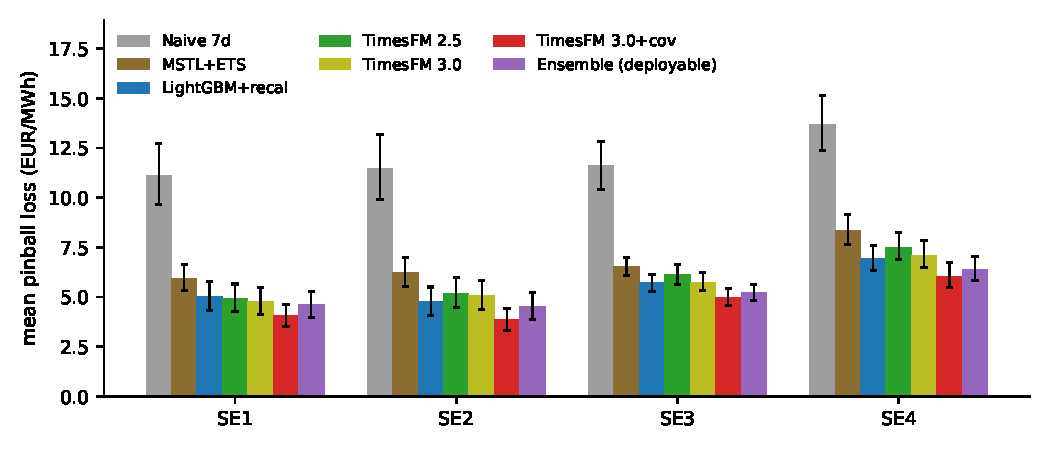
\includegraphics[width=\linewidth]{zone_scores}
\caption{Mean pinball loss per zone and model over the evaluation year, with 95\%
block-bootstrap confidence intervals.}
\label{fig:zones}
\end{figure}

\begin{itemize}
\item \textbf{TimesFM 3.0 with covariates is the best model in every zone}, 12--20\% better than
LightGBM (DM $p<0.001$ everywhere), and its intervals are close to nominal without any
recalibration (coverage 76--80\% / 86--88\%). Without covariates, 3.0 is roughly level with
LightGBM: the covariates matter.
\item \textbf{TimesFM 2.5 alone is worse than LightGBM} in SE2--SE4 and level in SE1. Adding XReg
covariates made 2.5 \emph{worse}; a linear in-context regression does not capture the
weather--price relation. Recalibration does not help either TimesFM model.
\item \textbf{The errors are complementary} (Figure~\ref{fig:hourly}). TimesFM~2.5, and even MSTL,
beat LightGBM clearly in the first hours of the delivery day: models that read the series up to its
last published hour (23:00 on day $D$) carry the overnight level forward, whereas LightGBM's
nearest same-hour lag is 24 hours old. LightGBM wins from the morning ramp onwards and on spike
days, where weather drives prices.
\end{itemize}

\begin{figure}[h]
\centering
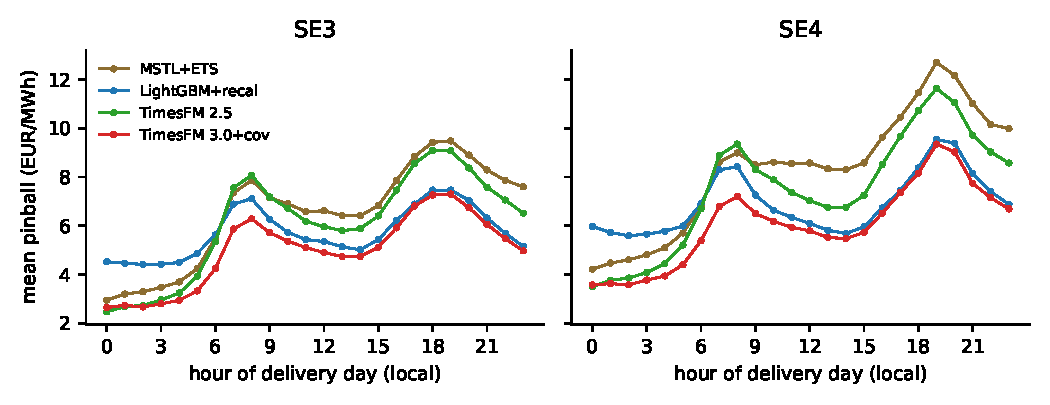
\includegraphics[width=\linewidth]{hourly}
\caption{Mean pinball loss by hour of the delivery day.}
\label{fig:hourly}
\end{figure}

\begin{figure}[h]
\centering
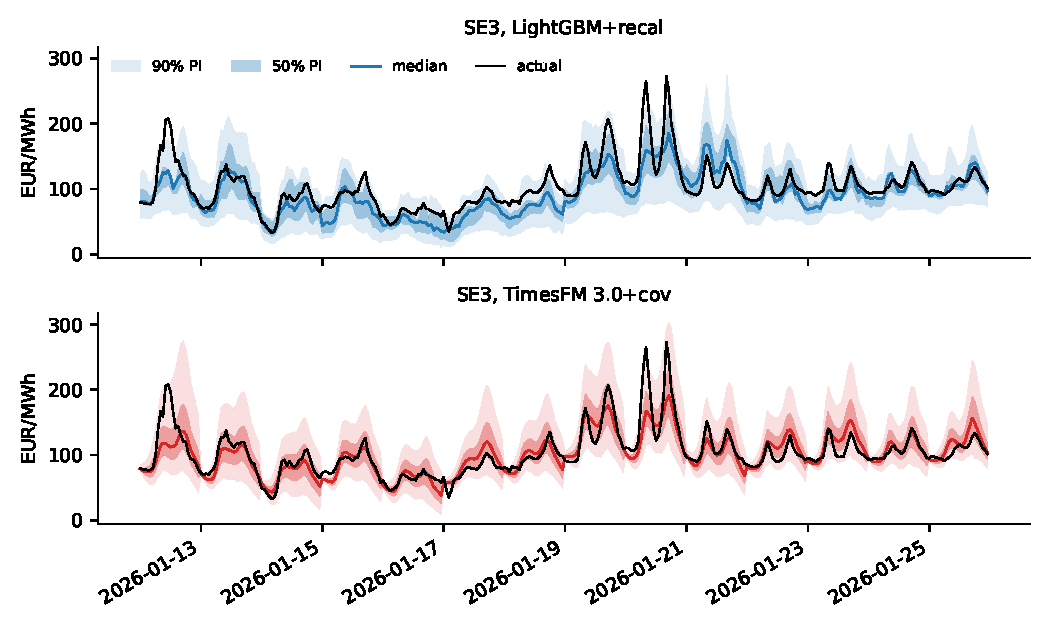
\includegraphics[width=\linewidth]{fan}
\caption{Two winter weeks in SE3: 50\% and 90\% prediction intervals, median and actual price for
recalibrated LightGBM (top) and TimesFM 3.0 with covariates (bottom).}
\label{fig:fan}
\end{figure}

\subsection{Fine-tuning decision}
Fine-tuning on a rented GPU is deferred. TimesFM~3.0 already wins but cannot be deployed, and a
fine-tune would inherit its licence. TimesFM~2.5 meets the specification's precondition (better on
some slices), but combining it with LightGBM costs nothing and should be tried first. Fine-tuning
2.5 will only be proposed, with a cost estimate for the owner's approval, if a clear gap to
TimesFM~3.0 remains after the ensemble.

%------------------------------------------------------------------------------
\section{Ensemble (M8)}

\subsection{Design}
The ensemble is one more \code{Forecaster} in the harness, so it is evaluated under exactly the
same conditions as its members. At each origin its members are refit on their own cadence and
forecast as usual; the ensemble forecast is a convex combination of their sorted quantiles,
\begin{equation}
\hat q^{\,\mathrm{ens}}_{\tau,t} = \sum_{k} w_{k,g(t)}\,\hat q^{(k)}_{\tau,t}, \qquad
w_{\cdot,g} \in \Delta^{K-1},
\end{equation}
where $g(t)$ is the weight group of target hour $t$: a single group (\emph{global}) or the local
hour of the delivery day (\emph{hourly}). Weights are chosen on a simplex grid (step 0.05) by
minimising mean pinball loss over the members' \emph{own past forecasts} of days that are
published by the origin, over a trailing 56-day or an expanding window. Until 14 days of
history exist the weights are equal. As with recalibration, realised prices reach the ensemble
only through the harness's published-before-origin training rows, so it cannot see the future.
The deployable ensemble combines the recalibrated LightGBM and TimesFM~2.5; a research variant
adds TimesFM~3.0 with covariates and is tagged non-deployable automatically, because an ensemble
is deployable only if all its members are.

\subsection{Results}

\begin{table}[h]
\centering\small
\caption{Ensembles, 365 origins per zone: mean pinball loss (EUR/MWh); paired difference of the
hourly expanding-window ensemble to LightGBM with 95\% block-bootstrap CI (DM $p<0.001$ in every
zone). The research ensemble includes TimesFM~3.0 and is not deployable.}
\label{tab:ensemble}
\footnotesize\setlength{\tabcolsep}{3.5pt}
\begin{tabular}{lcccccc|cc}
\toprule
& & \multicolumn{3}{c}{deployable ensemble} & & & \multicolumn{2}{c}{research only}\\
\cmidrule(lr){3-5}\cmidrule(lr){8-9}
Zone & LGBM+recal & equal & hourly 56d & hourly exp. & $\Delta$ [95\% CI] & Cov.\ 80/90 & ens.\ +3.0 & 3.0+cov\\
\midrule
SE1 & 5.053 & 4.701 & 4.630 & \best{4.608} & $-0.45$ [$-0.61$, $-0.29$] & 79.5/88.8 & 4.086 & 4.054\\
SE2 & 4.788 & 4.690 & 4.552 & \best{4.528} & $-0.26$ [$-0.35$, $-0.17$] & 79.8/89.3 & 3.883 & 3.866\\
SE3 & 5.727 & 5.430 & 5.273 & \best{5.248} & $-0.48$ [$-0.60$, $-0.36$] & 81.6/90.1 & 4.873 & 4.989\\
SE4 & 6.920 & 6.581 & 6.408 & \best{6.390} & $-0.53$ [$-0.67$, $-0.38$] & 82.2/90.4 & 5.964 & 6.059\\
\bottomrule
\end{tabular}
\end{table}

\begin{itemize}
\item \textbf{Per-hour weights are what matters.} Equal weights already help (except in SE2,
where the gain is not significant), global weights add nothing over equal weights, and hourly
weights roughly double the gain. The expanding window is marginally better than 56 days.
\item \textbf{The learnt weights are interpretable and stable} (Figure~\ref{fig:weights}):
TimesFM~2.5 receives 0.7--1.0 in hours 0--5, where it carries the last published price level
forward, and 0.05--0.6 from hour 7 onwards, where LightGBM's weather drivers dominate (SE1 keeps the
most TimesFM weight). In SE3 the mid-year and final weights differ by at most 0.1.
\item \textbf{No degradation where it matters.} Spike days improve in every zone (by 1--9\%);
the only worse slice is SE1 negative-price hours (+6\%, a small slice). Interval coverage stays
within 2.5 points of nominal.
\item \textbf{Gap to the benchmark.} The deployable ensemble closes 65\% (SE3), 61\% (SE4),
45\% (SE1) and 28\% (SE2) of the gap between LightGBM and TimesFM~3.0 with covariates. Adding
TimesFM~3.0 to the ensemble matches or beats TimesFM~3.0 alone, but is not deployable.
\end{itemize}

\begin{figure}[h]
\centering
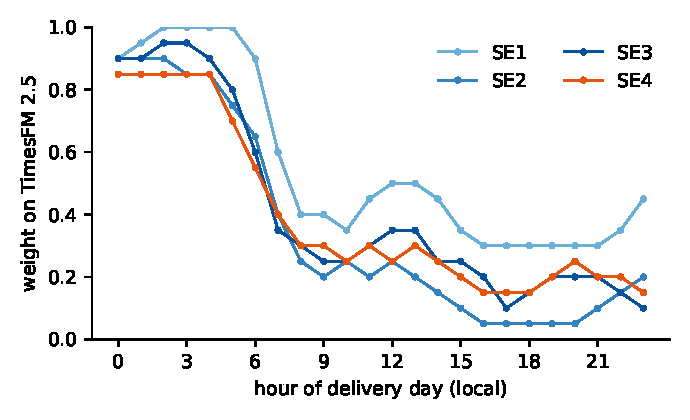
\includegraphics[width=0.6\linewidth]{weights}
\caption{Learnt ensemble weight on TimesFM~2.5 by hour of the delivery day (final weights
of the evaluation year; LightGBM receives the complement).}
\label{fig:weights}
\end{figure}

By the promotion criteria, the hourly expanding-window ensemble of recalibrated LightGBM and
TimesFM~2.5 replaces LightGBM as the champion candidate in every zone.

%------------------------------------------------------------------------------
\section{Issues found and fixed along the way}

{\small\noindent
\begin{tabularx}{\linewidth}{>{\raggedright\arraybackslash}p{4.2cm}X}
\toprule
Issue & Resolution\\
\midrule
Source shifted hours on 5 days & Verified against Energy-Charts; excluded via \code{known\_bad\_days}, never repaired.\\
Open-Meteo \code{best\_match} switches models & Pinned ECMWF IFS for training and evaluation.\\
Day-1 weather lead arrives after the origin & Day-2 lead with explicit availability rule.\\
Holiday names depend on system locale & Language pinned; test under three locales.\\
Development sample hit only Saturdays & Stride 5 by default; multiples of 7 rejected.\\
Model variants overwrote each other in comparisons & Keyed by full variant spec; regression test.\\
\code{predict} received the target column & Harness strips target and metadata; test.\\
Raw LightGBM over-confident on live weather & Rolling 28-day quantile recalibration.\\
TimesFM clamped forecasts at zero & \code{infer\_is\_positive} disabled.\\
LightGBM + torch OpenMP deadlock (macOS) & Torch limited to one thread.\\
Ensemble member specs invalid as MLflow names & Sanitised; test against MLflow's validator.\\
\bottomrule
\end{tabularx}\par}

%------------------------------------------------------------------------------
\section{Conclusions and next steps}

\begin{enumerate}
\item A leakage-audited, fully versioned pipeline produces calibrated quantile forecasts for all
four zones, with every number in this report traceable to an MLflow run.
\item The tuned, recalibrated LightGBM is 13--23\% better than MSTL and 49--58\% better than the
seasonal naive reference, significant in every zone.
\item TimesFM~3.0 with covariates shows a further 12--20\% of headroom, but only as a
non-deployable benchmark.
\item TimesFM~2.5 and LightGBM make complementary errors. Their hourly-weighted ensemble is the
deployable champion candidate: a further 5--9\% better than LightGBM in every zone, closing
28--65\% of the gap to TimesFM~3.0 without licence restrictions.
\item A cheap LightGBM improvement follows from Figure~\ref{fig:hourly}: features describing the
last published hours of day $D$ should fix its night-hour weakness.
\item M6 will wrap the ensemble (both members, weights and recalibration state) for the MLflow
registry and serve the daily 09:00 forecast. Fine-tuning TimesFM~2.5 remains deferred: the
remaining gap of 0.4--0.7~EUR/MWh does not yet justify GPU spend.
\end{enumerate}

%------------------------------------------------------------------------------
\appendix
\section{Reproducing the results}
\begin{verbatim}
uv sync --extra timesfm                       # environment from the lockfile
uv run python -m pricefc ingest prices        # elprisetjustnu.se, resumable
uv run python -m pricefc ingest weather       # Open-Meteo ECMWF IFS
uv run python -m pricefc dataset build stitched -z SE3
uv run python -m pricefc dataset build true_lead -z SE3
uv run python -m pricefc tune -z SE3          # Optuna, before eval year
uv run python -m pricefc backtest run -z SE3 \
    -m mstl_ets -m "lightgbm_tuned_SE3@calibration=28" \
    -m timesfm25 -m timesfm3_cov
uv run python -m pricefc backtest run -z SE3 -m ensemble_hourly_exp
uv run python -m pricefc backtest compare <run ids> --reference mstl_ets
uv run python docs/report/make_figures.py     # figures in this report
\end{verbatim}
Dataset versions used: stitched \code{20261004-*} and true-lead \code{20261004-*} per zone
(SE3: \code{959ffb} and \code{220df7}). The decision log \code{docs/decisions.md} records every
choice with its date and evidence.

\end{document}
